\subsection{XDP}

\begin{frame}{eXpress Data Path}
	\begin{itemize}
		\item Run an eBPF program as close to frame reception as possible
		\item Support is Hardware-specific and driver-specific
		\item Introduced for high-performance networking, but available on embedded devices
		\item Take very fast decisions in the driver, with user-configurable eBPF code
		\item Used for fast routing, DDoS protection, firewalling, etc.
		\item With \code{AF_XDP}, offers an upstream alternative to kernel bypass
	\end{itemize}
\end{frame}

\begin{frame}{XDP program}
	\begin{columns}
		\column{0.3\textwidth}
		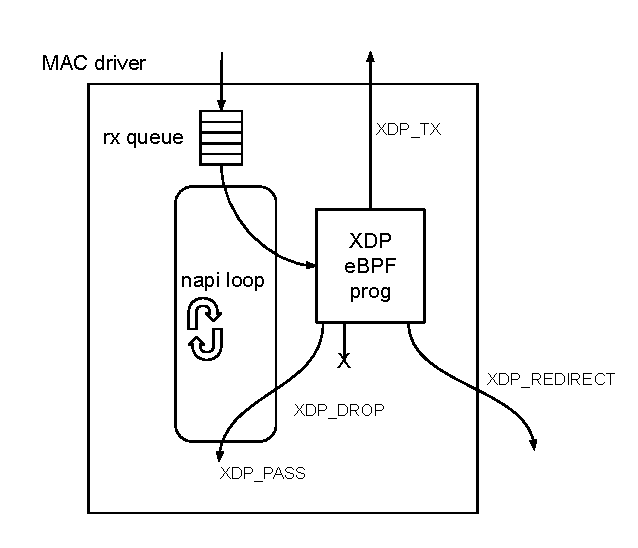
\includegraphics[width=1.4\textwidth]{slides/networking-ebpf-xdp/xdp.pdf}
		\column{0.7\textwidth}
	\begin{itemize}
		\item XDP programs are run by the MAC driver in the NAPI loop
		\item XDP programs may edit the received frame, and take a decision :
			\begin{itemize}
				\item \code{XDP_PASS} : Packet continues to the Networking stack
				\item \code{XDP_DROP} : Packet is immediately dropped
				\item \code{XDP_ABORTED} : Similar \code{XDP_DROP} but triggers a \href{https://elixir.bootlin.com/linux/v6.12.32/A/ident/xdp_exception}{tracepoint}
				\item \code{XDP_TX} : Packet is sent back from the same interface
				\item \code{XDP_REDIRECT} : Packet is sent either :
					\begin{itemize}
						\item back from another interface
						\item to another CPU for processing
						\item to an \code{AF_XDP} socket
					\end{itemize}
			\end{itemize}
	\end{itemize}
	\end{columns}
\end{frame}

\begin{frame}[fragile]{XDP hook - driver side}
	\begin{minted}{c}
u32 bpf_prog_run_xdp(const struct bpf_prog *prog, struct xdp_buff *xdp);
	\end{minted}
		\vspace{0.6cm}
	\begin{columns}
	\column{0.3\textwidth}
		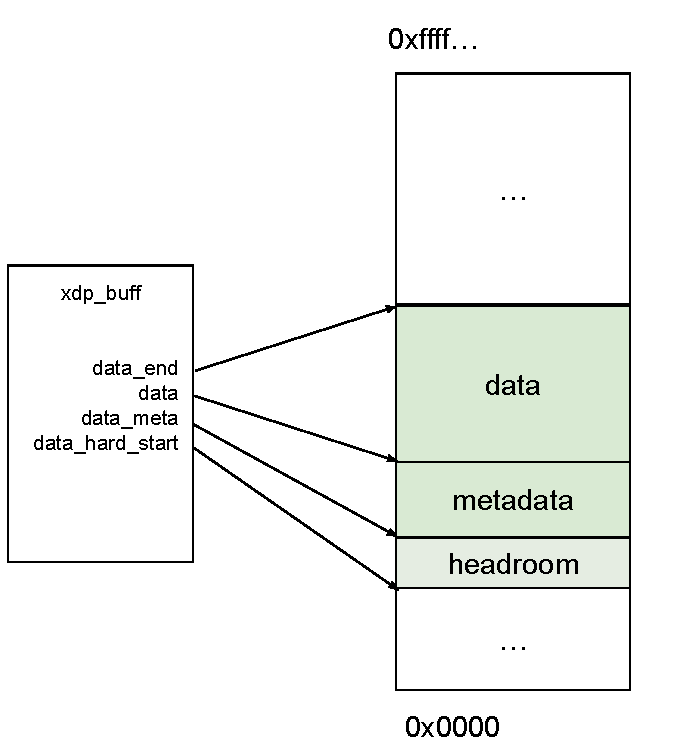
\includegraphics[width=1.3\textwidth]{slides/networking-ebpf-xdp/xdp_buff.pdf}
	\column{0.7\textwidth}
	\begin{itemize}
		\item \kstruct{bpf_prog} : The XDP program attached to the interface
		\item \kstruct{xdp_buff} : A representation of the buffer
		\item XDP runs \textit{before} the \code{skb} is even created
		\item a \kstruct{xdp_buff} is a very simple and lightweight representation of a frame
	\end{itemize}
	\end{columns}
\end{frame}

\begin{frame}[fragile]{XDP hook - eBPF side}
	\begin{block}{\href{https://elixir.bootlin.com/linux/v6.12.32/source/tools/testing/selftests/bpf/progs/xdp_dummy.c}{example program}}
		{\fontsize{8}{9}
	\begin{minted}{c}
SEC("xdp")
int xdp_dummy_prog(struct xdp_md *ctx)
{
        return XDP_PASS;
}
	\end{minted}
		}
	\end{block}
	\begin{block}{\kstruct{xdp_md} definition}
		{\fontsize{8}{9}
	\begin{minted}{c}
struct xdp_md {
        __u32 data;
        __u32 data_end;
        __u32 data_meta;
        __u32 ingress_ifindex; /* rxq->dev->ifindex */
        __u32 rx_queue_index;  /* rxq->queue_index  */
        __u32 egress_ifindex;  /* txq->dev->ifindex */
};
	\end{minted}
		}
	\end{block}

\end{frame}

\begin{frame}[fragile]{XDP\_DROP}
	\begin{itemize}
		\item Used for firewalling and DDoS protection
		\item A XDP Program returning \code{XDP_DROP} causes the frame to be dropped immediately
		\item \code{XDP_ABORTED} is similar, but triggers a tracepoint.
		\item Happens before the \kstruct{sk_buff} is even created
		\item If the driver uses \code{page_pool}, the buffer is recycled
		\item Extremely efficient way of filtering
	\end{itemize}
\end{frame}

\begin{frame}{XDP\_PASS}
	\begin{itemize}
		\item A XDP Program returning \code{XDP_PASS} causes the frame to continue through the network stack
		\item The XDP program may modify the frame
		\item After \code{XDP_PASS}, a \kstruct{sk_buff} will be created by the MAC driver
		\item The usual processing of the packet through the stack will occur
	\end{itemize}
\end{frame}

\begin{frame}{XDP\_TX}
	\begin{columns}
	\column{0.3\textwidth}
		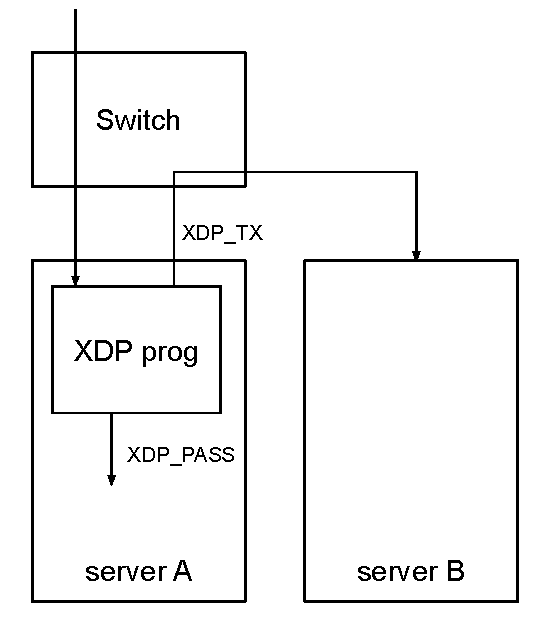
\includegraphics[width=\textwidth]{slides/networking-ebpf-xdp/xdp_lb.pdf}
	\column{0.7\textwidth}
	\begin{itemize}
		\item A XDP Program returning \code{XDP_TX} re-emits the frame on the same interface
		\item The frame may be modified by the program
		\item Main advertised use-case is to perform load-balancing
	\end{itemize}
	\end{columns}
\end{frame}

\begin{frame}[fragile]{XDP\_REDIRECT}
	\begin{itemize}
		\item Redirects the frame towards a target identified by a \textbf{map}
		\item Programs don't directly return \code{XDP_REDIRECT}
		\item The special bpf helper \code{bpf_redirect_map()} must be used
			\begin{itemize}
				\item See \manpage{bpf-helpers}{7}
			\end{itemize}
	\end{itemize}
	\begin{block}{\href{https://elixir.bootlin.com/linux/v6.15.1/source/tools/testing/selftests/bpf/progs/xdp_redirect_map.c}{Example XDP redirect}}
		{\fontsize{8}{9}
		\begin{minted}{c}
struct {
        __uint(type, BPF_MAP_TYPE_DEVMAP);
        __uint(max_entries, 8);
        __uint(key_size, sizeof(int));
        __uint(value_size, sizeof(int));
} tx_port SEC(".maps");

SEC("xdp")
int xdp_redirect_map_0(struct xdp_md *xdp)
{
        return bpf_redirect_map(&tx_port, 0, 0);
}
		\end{minted}
		}
	\end{block}
\end{frame}

\begin{frame}[fragile]{\code{bpf_redirect_map}}
	\begin{minted}{c}
long bpf_redirect_map(void *map, __u64 key, __u64 flags)
	\end{minted}
	\begin{itemize}
		\item See \manpage{bpf-helpers}{7}
		\item eBPF helper for \code{XDP_REDIRECT} actions
		\item The redirection target is \code{map[key]}, where \code{map} can be :
			\begin{itemize}
				\item A \ksym{BPF_MAP_TYPE_DEVMAP}, value is an \code{ifindex}
				\item A \ksym{BPF_MAP_TYPE_CPUMAP}, value is a \code{cpu number}
				\item A \ksym{BPF_MAP_TYPE_XSKMAP}, value is a \code{queue index}
			\end{itemize}
	\end{itemize}
\end{frame}

\begin{frame}{XDP\_REDIRECT - To device}
	\begin{columns}
	\column{0.3\textwidth}
		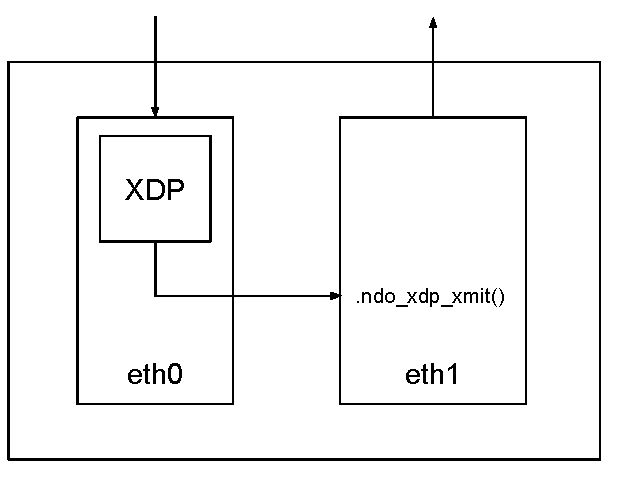
\includegraphics[width=\textwidth]{slides/networking-ebpf-xdp/xdp_redirect_devmap.pdf}
	\column{0.7\textwidth}
	\begin{itemize}
		\item Uses \ksym{BPF_MAP_TYPE_DEVMAP}, Documented \href{https://docs.kernel.org/bpf/map_devmap.html}{here}
		\item Forwards the frame to another XDP-enabled \kstruct{net_device}
		\item The target device must implement \code{.ndo_xdp_xmit()}
		\item No \kstruct{sk_buff} is created, the \kstruct{xdp_buff} is sent directly
		\item \code{bpf_redirect()} can be used directly
	\end{itemize}
	\end{columns}
\end{frame}

\begin{frame}{XDP\_REDIRECT - To CPU}
	\begin{columns}
	\column{0.4\textwidth}
		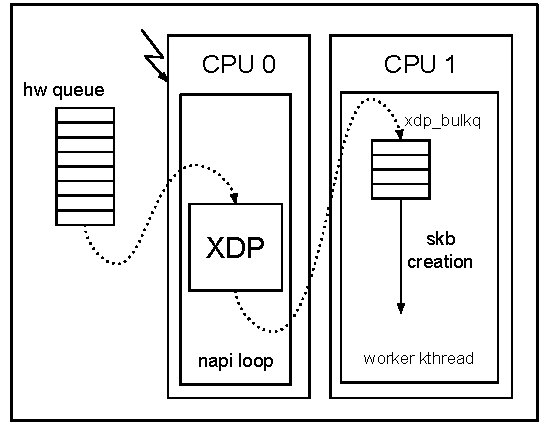
\includegraphics[width=\textwidth]{slides/networking-ebpf-xdp/xdp_redirect_cpumap.pdf}
	\column{0.6\textwidth}
	\begin{itemize}
		\item Uses \ksym{BPF_MAP_TYPE_CPUMAP}, Documented \href{https://docs.kernel.org/bpf/map_cpumap.html}{here}
		\item Make the packet processing occur on another CPU core
		\item Useful for CPU load balancing
		\item Also used to circumvent hardware issues
			\begin{itemize}
				\item Flawed hash computation in hardware for RSS
				\item Wrong internal \href{https://elixir.bootlin.com/linux/v6.15.1/source/drivers/net/ethernet/marvell/mvneta.c\#L4424}{interrupt routing}
			\end{itemize}
	\end{itemize}
	\end{columns}
\end{frame}

\begin{frame}{XDP\_REDIRECT - To Socket}
	\begin{columns}
	\column{0.4\textwidth}
		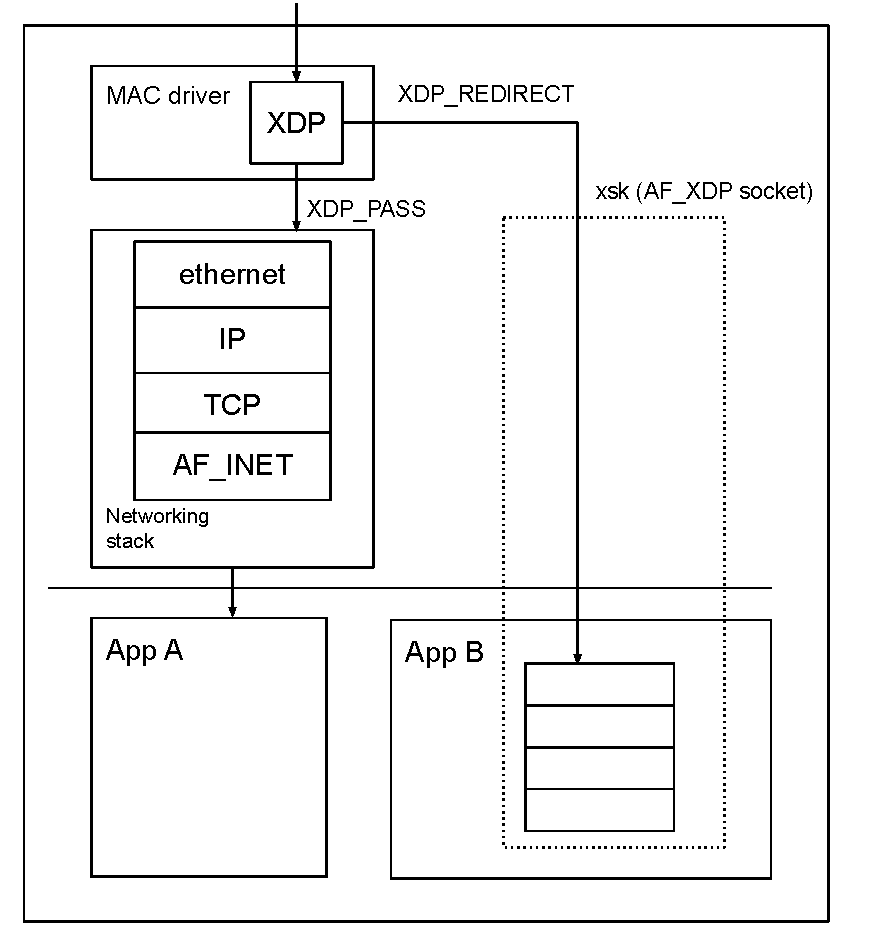
\includegraphics[width=\textwidth]{slides/networking-ebpf-xdp/xdp_redirect_xskmap.pdf}
	\column{0.6\textwidth}
	\begin{itemize}
		\item Uses \ksym{BPF_MAP_TYPE_XSKMAP}, Documented \href{https://docs.kernel.org/bpf/map_xskmap.html}{here}
		\item Frames are forwarded directly to user memory attached to an \ksym{AF_XDP} socket (\textbf{XSK})
		\item Upstream Linux's response to out-of-tree kernel bypass (e.g. DPDK)
		\item The driver is still in kernel, and the XDP program choses if bypass is needed for each frame
		\item No copy occurs, a \textbf{dedicated hardware queue} is needed
		\item Memory is shared with the \textbf{UMEM}, bound to a \code{queue_id} with \code{bind()}
		\item UMEM regions are shared ring-buffers, where user buffers are directly mapped to hw queues
	\end{itemize}
	\end{columns}
\end{frame}

\begin{frame}{XDP support in a driver}
	\begin{enumerate}
		\item Implement the execution and return-code handling of the BPF XDP programs
			\begin{itemize}
				\item Fairly straightforward, done in the main NAPI loop
			\end{itemize}
		\item Make sure the data handling meets the following constraints :
			\begin{itemize}
				\item Frame must be \textbf{readable} and \textbf{writeable}
				\item There must be \textbf{a headroom} big enough to fit \code{struct xdp_frame}
				\item There must be \textbf{a tailroom} big enough to fit all \code{skb_shared_info}
			\end{itemize}
		\item \href{https://lore.kernel.org/netdev/cover.1642758637.git.lorenzo@kernel.org/}{XDP frags} is supported since v5.16
			\begin{itemize}
				\item Allows using XDP with non-linear frames, which used to be impossible
			\end{itemize}
		\item The \kstruct{xdp_buff} layout uses \kstruct{skb_frag} as well
	\end{enumerate}
\end{frame}

\begin{frame}[fragile]{Loading an XDP program}
	\begin{itemize}
		\item XDP programs are built like any other eBPF program :
			\begin{minted}{console}
clang -O2 -g -target bpf -c xdp_prog.c -o xdp_prog.o
			\end{minted}
		\item They can be loaded with \code{iproute2} :
			\begin{minted}{console}
ip link set dev eth0 xdp obj xdp-prog.o
			\end{minted}
		\item \code{iproute2} xdp support is recent, \code{xdp-loader} from \code{xdp-tools} can be used :
			\begin{minted}{console}
xdp-loader load eth0 xdp_drop.o
			\end{minted}
		\item \code{bpftool} can also be used to attach XDP programs
		\item \code{ethtool -S <iface>} shows the XDP statistics
		\item \code{xdp-monitor} shows detailed statistics using BPF tracing

	\end{itemize}
\end{frame}


% XDP presentation
% Writing XDP

